\chapter{如何解决一些现实问题}

\section{如何解决查新的问题}

由于查新仅仅是通过字符串匹配的问题,所以只要把文中的字符复制到Word里面即可,不用考虑格式的问题。下面提供几种将pdf文件转成word格式的方法,所有内容来自善用佳软上的文章\textbf{PDF转换word格式的方法总结}(\url{http://xbeta.info/pdf2word.htm})。

\subsection{推荐的PDF转换word方案}

PDFtoWord.com(\url{http://www.pdftoword.com/}) 号称是目前最为精准的pdf to word文件转换器,出自著名的PDF解决方案供应商NitroPDF。PDFtoWord.com是在线应用,完全免费,使用方便:
\begin{enumerate}
\item 访问pdftoword.com
\item 上传pdf
\item 输入接收邮箱
\item 进入邮箱:查收转换后的word文档。
\end{enumerate}
推荐这个网站的原因是这个网站对中文的支持非常好,而且Pdftoword 在排版方面确实有独到之处,特别介绍一个细节,Pdftoword 转换后的文档仍以段落为单位,没有很多的换行符,而以前大多转换器都是以行为单位,以致末尾有很多的换行符,你复制粘贴时会有许多麻烦。

\newpage

\section{如何绘制表格}

\subsection{比较好用的转换工具}
关于如何绘制表格,tex@stackexchange (\url{http://tex.stackexchange.com/}) 上面有一个非常全面的 帖子(\url{http://tex.stackexchange.com/questions/49414/comprehensive-list-of-tools-that-simplify-the-generation-of-latex-tables}),帖子里面介绍的内容应该是市面上最全面的了。

推荐两款软件:
\begin{itemize}
\item excel2latex
\item Calc2LaTeX
\end{itemize}

\subsubsection{excel2latex}

下载地址( \url{http://www.ctan.org/tex-archive/support/excel2latex/})

使用起来很简单,下载之后双击\texttt{Excel2LaTeX.xla} 文件就能在Excel中看到一个加载项标签,然后点击按钮就会得到相应的LaTeX命令,复制到LaTeX文件里面就好了。

\subsubsection{Calc2LaTeX}

Calc2LaTeX
\url{http://calc2latex.sourceforge.net/} 需要安装开源的OpenOffice,如果你是在linux下面使用这个模板,那么就需要用到OpenOffice了(当然了,在Windows下面也可以使用)。

1 Click 'Tools'-'Macros'-'Organize Macros'-'OpenOffice.org Basic...'. 
\begin{figure}[h]
\centering
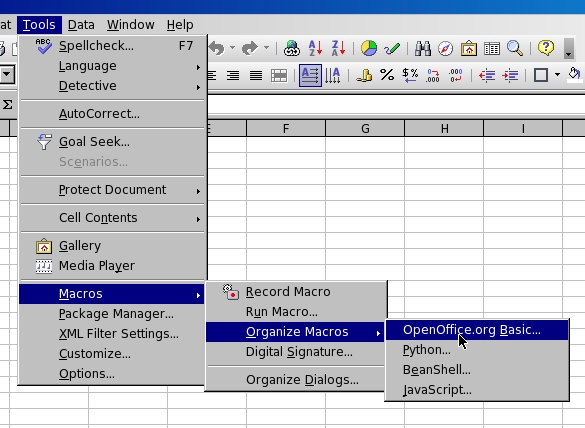
\includegraphics[scale=0.4]{figs/step1_oo20}
\end{figure}

2 You will see 'OpenOffice.org Basic Macros' dialog box. Select 'My Macros' and push 'Organizer' button.
\begin{figure}[h]
\centering
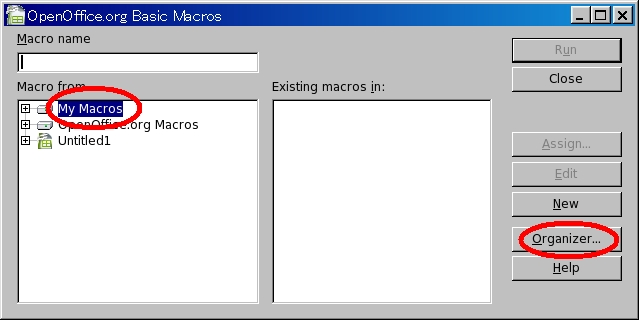
\includegraphics[scale=0.4]{figs/step2_oo20}
\end{figure}

3 Click 'Libraries' tab, and confirm that 'My Macros \& Dialogs' is selected on the list of 'Location.' (If not, select it.) And then click 'Append' button.
\begin{figure}[h]
\centering
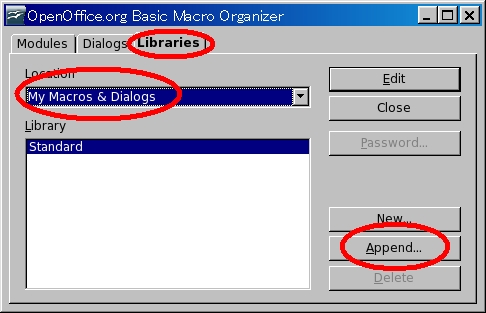
\includegraphics[scale=0.4]{figs/step3_oo20}
\end{figure}

4 You will see a file dialog, so select 'script.xlb' which you have extracted from the zip file in advance.
\begin{figure}[h]
\centering
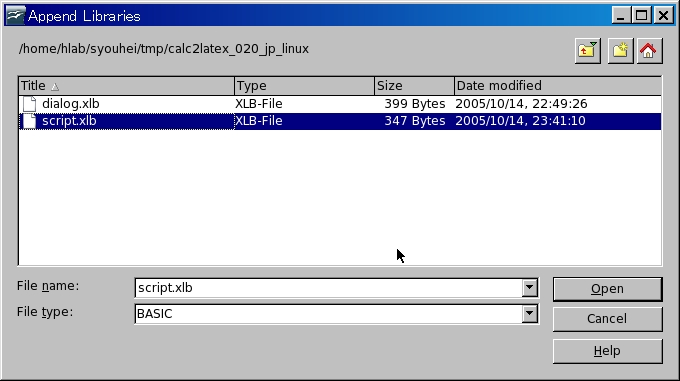
\includegraphics[scale=0.4]{figs/step4_oo20}
\end{figure}

5 'Append Libraries' dialog box will show. Check 'Calc2LaTeX', and push 'OK'.
If you want to update Calc2LaTeX on your machine, check 'Replace existing libraries' option.
\begin{figure}[h]
\centering
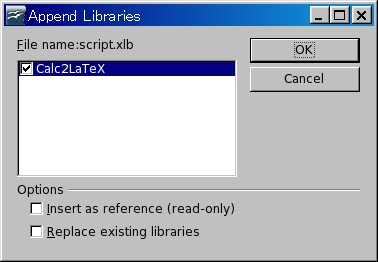
\includegraphics[scale=0.4]{figs/step5_oo20}
\end{figure}

6 That's all. You can close dialog boxes opened in above-mentioned steps. And also you can delete the zip file and the extracted files.
Enjoy Calc2LaTeX!

Usage

\begin{enumerate}
\item Run OpenOffice Calc.
\item Select cells you want to convert into LaTeX format.
\item Push 'Tools'-'Macro'. (In the case of OpenOffice1.1 RC, push 'Tools'-'Macros'-'Macro')
\item You will see 'Macro' dialog box. And then click 'soffice'-'calc2latex' in Macro form to show 'Main' item.
\item Select 'Main' in 'soffice'-'calc2latex'-'Main' and push 'Run' button.
\end{enumerate}

After these steps...
To get results, select all strings in 'Results' dialog box, and copy them to clipboard (push right buttom of mouse and push 'copy' in Windows environments).

\subsection{表格特别长怎么办}

用\texttt{tabu}宏包提供的命令,比如表\ref{tbl:4}特别的宽,用\texttt{tabu}中的 \texttt{to\linewidth} 命令
就可以把表格内容自动限定在页面宽度内,当然了,下面的表格也使用了\texttt{\footnotesize}来缩小表格的字号

表格\ref{tbl:4}的命令如下:
\begin{verbatim}
\begin{table}
\begin{tabu} to\linewidth {|X[4c]|X[1.5c]|X|X|X[1.5c]|X|X|X[1.5c]|X|X|}
\hline
\rowfont [c]\footnotesize
\multicolumn{ 1}{|c|}{Attacks} & \multicolumn{3}{c|}{Mandrill}
 & \multicolumn{ 3}{c|}{Lena}& \multicolumn{ 3}{c|}{Peppers} 
 \\ \cline{ 2- 10}
 
\rowfont [c]\footnotesize
\multicolumn{ 1}{|c|}{} & Proposed Scheme & Scheme  & Scheme in  
& Proposed Scheme & Scheme in  & Scheme in  & Proposed Scheme & 
Scheme in  & Scheme in  \\ \hline
...... 
省略中间的内容
Rotation 30 degrees & 5/10 & 4/15 & 0/8 & 6/12 & 4/10 & 2/8 & 
8/13 & 7/23 & 1/8 \\ \hline
\end{tabu}
\TableBicaption{特别宽的表格}{A really wide table}
\label{tbl:4}
\end{table}
\end{verbatim}



\begin{table}
\begin{tabu} to\linewidth {|X[4c]|X[1.5c]|X|X|X[1.5c]|X|X|X[1.5c]|X|X|}
\hline
\rowfont [c]\footnotesize
\multicolumn{ 1}{|c|}{Attacks} & \multicolumn{3}{c|}{Mandrill} & \multicolumn{ 3}{c|}{Lena} & \multicolumn{ 3}{c|}{Peppers} \\ \cline{ 2- 10}
\rowfont [c]\footnotesize
\multicolumn{ 1}{|c|}{} & Proposed Scheme & Scheme  & Scheme in  & Proposed Scheme & Scheme in  & Scheme in  & Proposed Scheme & Scheme in  & Scheme in  \\ \hline

Centered cropping 5\% off & 10/10 & 6/15 & 4/8 & 12/12 & 7/10 & 5/8 & 13/13 & 6/23 & 2/8 \\ \hline
Centered cropping 10\% off & 9/10 & 5/15 & 2/8 & 11/12 & 5/10 & 3/8 & 11/13 & 5/23 & 2/8 \\ \hline
Scaling 50\% & 5/10 & 4/15 & 0/8 & 6/12 & 1/10 & 2/8 & 7/13 & 2/23 & 3/8 \\ \hline
Scaling 90\% & 6/10 & 3/15 & 2/8 & 9/12 & 2/10 & 3/8 & 10/13 & 5/23 & 4/8 \\ \hline
Scaling 150\% & 5/10 & 6/15 & 1/8 & 7/12 & 4/10 & 3/8 & 8/13 & 6/23 & 3/8 \\ \hline
aspect ratio changing (0.9, 1.0) & 5/10 & 1/15 & 0/8 & 8/12 & 4/10 & 0/8 & 8/13 & 4/23 & 0/8 \\ \hline
aspect ratio changing (1.0, 1.1) & 6/10 & 2/15 & 0/8 & 10/12 & 6/10 & 0/8 & 9/13 & 7/23 & 0/8 \\ \hline
Rotation 1 degrees & 8/10 & 6/15 & 3/8 & 8/12 & 3/10 & 5/8 & 11/13 & 9/23 & 3/8 \\ \hline
Rotation 5 degrees & 7/10 & 4/15 & 3/8 & 8/12 & 3/10 & 3/8 & 10/13 & 9/23 & 3/8 \\ \hline
Rotation 30 degrees & 5/10 & 4/15 & 0/8 & 6/12 & 4/10 & 2/8 & 8/13 & 7/23 & 1/8 \\ \hline
\end{tabu}
\TableBicaption{特别宽的表格}{A really wide table}
\label{tbl:4}
\end{table}


\section{如果忘了\LaTeX 命令怎么写该怎么办?}

\url{http://www.biwako.shiga-u.ac.jp/sensei/kumazawa/texindex3.html#formula}

\section{避免常见的\LaTeX 错误}

\begin{itemize}
\item Journal of Machine Learning Research 对于论文投稿论文的一些要求 (\url{http://jmlr.csail.mit.edu/format/format.html})
\item 有关中文本地化的内容
\item LATEX for Complete Novices \url{www.dickimaw-books.com/latex/novices/} 
\end{itemize}

\begin{description}

\item[破折号] 在句子中使用\raisebox{0.5mm}{---}破折号\raisebox{0.5mm}{---}达到插入效果的时候要特别小心。
破折号要长,并且在破折号之前和之后的都不应该有空格。
并且中文的破折号与英文的破折号高度不一样,所以\LaTeX 原始输入为:
\begin{verbatim}
在句子中使用\raisebox{0.5mm}{---}破折号\raisebox{0.5mm}{---}达到插入效果的时候要特别小心。
\end{verbatim}
\item[小写名称及缩写名称]文中出现的领域名称,算法名称,方法名称等都应该使用小写字母,比如:cognitive science, reinforcement learning, principal components analysis。
当涉及到组织名,比如Cognitive Science Department,或者涉及专有名词,比如Markov decision processes, Gaussian densities, Bayes' rule时才需要大写。

后文反复提到的缩写名称应该在文中第一次提及时给出完整的英文全程和缩写,比如隐狄利克雷分配(Latent Dirichlet Allocation, LDA)。
这样,在后文就可以使用LDA指代隐狄利克雷分配了。
\item[拉丁缩写]首先,文中不鼓励使用拉丁缩写。建议使用中文替代,``i.e.'' 替换为“即”,``e.g.''替换为“例如”。如果你实在是要用拉丁缩写,一定要使用正确,即,在每个字母后面都要有一个半角句号。
\item[公式编号]当且仅当后文要引用这个公式的时候才为这个公式编号。
\item[参考文献标引]参考文献标引在文中并不是名词。下面的语句是不对的:
\begin{verbatim}
利用[34]的方法,我们如何如何
\end{verbatim}
正确的句式为:
\begin{verbatim}
利用Smith在文献[23]提出的方法,我们如何如何
\end{verbatim}
或者:
\begin{verbatim}
利用非线性降维方法[34],我们如何如何。
\end{verbatim}
\item[不要使用utilize这个词]
\item[不要在一个段落后马上加入子段落]在两个段落之间应该有链接句子,不允许出现下面的情况:
\begin{verbatim}
5. 实验结果

5.1 退化实验结果
\end{verbatim}
正确的格式为:
\begin{verbatim}
5. 实验结果

在这一章,我们首先描述了 blah, blah, blah

5.1 退化实验结果
\end{verbatim}
\item[float环境位置]All text references to a table should be by a number, not
by an introductory phrase such as ‘in the following table’.”
\item[unbreakable space] 
\begin{verbatim}
Figure~\ref{fig:single} shows some shapes.
\end{verbatim}
效果为:Figure~\ref{fig:single} shows some shapes.
\item[math mode] 当输入变量的时候,一定要在数学模式输入,比如 $x,y,z$,而不是x,y,z.
\item[数学公式引用] \verb \eqref{label} = \verb (\ref{label})
\item[eqnarray] Don’t use the \texttt{eqnarray} or \texttt{eqnarray*} environments. They’re obsolete
\item[数学模式中插入文字]
\begin{align*} 
y &= 2x + 2\\
\intertext{Using the distributive law:中文也可以}
&= 2(x+1)
\end{align*}
\begin{verbatim}
\begin{align*} 
y &= 2x + 2\\
\intertext{Using the distributive law:中文也可以}
&= 2(x+1)
\end{align*}
\end{verbatim}
\item[数学字体] \verb \mathcal{text}  只对大写字母起作用
\begin{table}[htbp]
\centering
\begin{tabular}{cc}
\hline 
Example Input & Corresponding Output \\ 
\hline
\verb$\mathrm{xyz}$& $\mathrm{xyz}$ \\ 
\verb$\mathsf{xyz}$& $\mathsf{xyz}$  \\ 
\verb$\mathtt{xyz}$& $\mathtt{xyz}$   \\ 
\verb$\mathit{xyz}$& $\mathit{xyz}$   \\ 
\verb$\mathbf{xyz}$& $\mathbf{xyz}$   \\ 
\verb$\mathcal{OXYZ}$& $\mathcal{OXYZ}$   \\ 
\hline 
\end{tabular} 
\end{table}
花体数学字体
\begin{table}
\centering
\begin{tabular}{cc}
\hline
Example Input  & Example Output \\ 
\hline
\verb$\mathbb{A+B=C}$  & $\mathbb{A+B=C}$ \\ 
\verb$\mathfrak{A+B=C}$  & $\mathfrak{A+B=C}$ \\ 
\verb$\boldsymbol{A+B=C}$  & $\boldsymbol{A+B=C}$ \\ 
\verb$\pmb{+-=}$ &    $\pmb{+-=}$\\ 
\hline 
\end{tabular} 
\end{table}
\item[希腊字母]

\begin{table}[htbp]
\caption{Lower Case Greek Letters}
\label{tab:greek}
\centering
\begin{tabular}{llllll}
{alpha} & $\alpha$ &
{beta} & $\beta$ &
{gamma} & $\gamma$ \\
{delta} & $\delta$  &
{epsilon} & $\epsilon$ &
{varepsilon} & $\varepsilon$\\
{zeta} & $\zeta$ &
{eta} & $\eta$ &
{theta} & $\theta$ \\
{vartheta} & $\vartheta$ &
{iota} & $\iota$ & 
{kappa} & $\kappa$ \\
{lambda} & $\lambda$ &
{mu} & $\mu$ &
{nu} & $\nu$ \\
{xi} & $\xi$ &
{pi} & $\pi$ &
{varpi} & $\varpi$\\
{rho} & $\rho$ &
{varrho} & $\varrho$ &
{sigma} & $\sigma$ \\
{varsigma} & $\varsigma$ &
{tau} & $\tau$ &
{upsilon} & $\upsilon$ \\
{phi} & $\phi$ &
{varphi} & $\varphi$ &
{chi} & $\chi$ \\
{psi} & $\psi$ &
{omega} & $\omega$ 
\end{tabular}
\end{table}

\begin{table}[htbp]
\caption{Upper Case Greek Letters}
\label{tab:Greek}
\centering
\begin{tabular}{llllll}
{Gamma} & $\Gamma$ &
{Delta} & $\Delta$ &
{Theta} & $\Theta$ \\
{Lambda} & $\Lambda$ &
{Xi} & $\Xi$ &
{Pi} & $\Pi$ \\
{Sigma} & $\Sigma$ &
{Upsilon} & $\Upsilon$ &
{Phi} & $\Phi$ \\
{Psi} & $\Psi$ &
{Omega} & $\Omega$
\end{tabular}
\end{table}


\end{description}







